\documentclass[UTF8]{ctexart}
\usepackage{geometry}
\usepackage{amsmath}
\usepackage{graphicx}
\usepackage{hyperref}

\geometry{a4paper, left=2.5cm, right=2.5cm, top=2.5cm, bottom=2.5cm}

\hypersetup{
    colorlinks=true,
    linkcolor=blue,
    filecolor=magenta,      
    urlcolor=cyan,
}

\title{\textbf{基于深度学习的高性能手写数字识别模型研究}}
\author{作者: (请填写您的姓名) \\ 学号: (请填写您的学号) \\ 专业: (请填写您的专业)}
\date{\today}

\begin{document}

\maketitle
\thispagestyle{empty}

\begin{abstract}
\noindent
本项目旨在研究并实现一个高性能的卷积神经网络(CNN)模型,以解决经典的 MNIST 手写数字识别任务,目标是使模型在标准测试集上的准确率超越 99.5\%。为达成此目标,本研究没有局限于传统的 LeNet-5 架构,而是设计并实现了一个更深、更现代的 CNN 模型。研究的核心贡献在于综合运用了一系列高级优化策略,包括:(1)构建了一个包含三个卷积块并采用自适应平均池化的深度网络结构;(2)实施了包含随机仿射变换(Random Affine)与随机擦除(Random Erasing)在内的复合数据增强策略;(3)应用了标签平滑损失函数(Label Smoothing Loss)以提升模型的泛化能力;(4)采用了分层学习率(Discriminative Learning Rates)与 AdamW 优化器;(5)集成了 OneCycle 学习率调度器与自动混合精度(AMP)训练以加速收敛并优化性能。实验结果表明,本研究提出的模型在经过 30 个周期的训练后,在 MNIST 测试集上取得了 \textbf{99.65\%} 的最高分类准确率,成功超越预设目标,验证了所采用的综合优化策略的有效性。\footnote{项目完整代码已在 GitHub 开源: \url{https://github.com/LeaderOnePro/AICourseEndingAssignment}}
\end{abstract}

\section{引言 (Introduction)}

手写数字识别是计算机视觉与模式识别领域的一项基础性任务。尽管该问题已有数十年的研究历史,但它至今仍是验证和迭代新型神经网络架构、损失函数及优化策略的理想"试验场"。其在邮政编码自动分拣、银行票据处理等商业场景中的广泛应用,也持续驱动着研究者们追求更高的识别精度和模型效率。

经典的 LeNet-5 [1] 模型为解决此问题提供了卷积神经网络的开创性思路。然而,随着深度学习理论与实践的飞速发展,一系列更强大的网络组件与训练策略应运而生。本项目旨在探索,通过系统性地集成这些现代技术,能够在多大程度上提升模型在 MNIST 任务上的性能极限。

本研究的主要贡献如下:
\begin{itemize}
    \item 设计并实现了一个深度卷积神经网络,其性能显著优于传统浅层网络。
    \item 综合运用了包括复合数据增强、标签平滑、分层学习率在内的多种高级训练技巧。
    \item 通过严谨的实验,验证了该综合优化方案的有效性,最终取得了超越 99.5\% 目标的高性能结果。
\end{itemize}

\section{方法论 (Methodology)}

为实现高性能的识别模型,我们从网络架构、数据处理、损失函数及训练策略四个方面进行了系统性设计。

\subsection{网络架构}

我们设计了一个名为 \texttt{ImprovedNet} 的深度卷积神经网络。与 LeNet-5 相比,该网络具有更强的特征提取能力和更现代的结构设计。其核心由三部分构成:

\begin{enumerate}
    \item \textbf{卷积特征提取模块 (\texttt{conv\_layers})}: 包含三个级联的卷积块。每个块由两个 \texttt{Conv2d} 层和一个 \texttt{BatchNorm2d} 层、\texttt{ReLU} 激活函数构成,并在块的末端使用 \texttt{MaxPool2d} 进行下采样和 \texttt{Dropout2d} 进行正则化。网络深度和宽度的增加(通道数从32 -> 64 -> 128)使其能学习从低阶到高阶的多层次特征。
    \item \textbf{自适应池化层 (\texttt{AdaptiveAvgPool2d})}: 在卷积模块的末端,我们使用自适应平均池化将不同尺寸的特征图统一降维到 1x1 大小。这使得网络对输入尺寸的变化更加鲁棒,并有效减少了从卷积层到全连接层的参数数量。
    \item \textbf{分类器模块 (\texttt{classifier})}: 由多个 \texttt{Linear} 层、\texttt{ReLU} 激活函数和 \texttt{Dropout} 组成,负责对提取到的高级特征进行最终的分类判决。
\end{enumerate}

\subsection{数据预处理与增强}

高质量的数据是训练高性能模型的基石。我们为训练集设计了一套丰富的在线数据增强(Data Augmentation)流水线:

\begin{itemize}
    \item \textbf{随机仿射变换}: 对图像进行 ±12度的随机旋转、±12\%的随机平移、±15\%的尺度缩放以及8度的剪切变换。这模拟了手写数字在现实中可能出现的各种形态变化,是提升模型泛化能力的基石。
    \item \textbf{随机擦除 (Random Erasing)}: 以 0.3 的概率,在图像上随机选取一个区域并用随机像素值进行覆盖。该策略模拟了数字图像中可能出现的局部遮挡。这种方式强制模型学习目标的全局结构,而非依赖于少数几个显著的局部特征,从而显著提升了模型的泛化能力与鲁棒性。
    \item 对于测试集,我们仅进行标准的张量转换与归一化,以保证评估结果的一致性与可复现性。
\end{itemize}

\subsection{损失函数:标签平滑}

传统的交叉熵损失函数使用 one-hot 编码的硬标签(hard labels)进行监督,这可能导致模型对训练数据过分自信(over-confident),降低其泛化能力。为解决此问题,我们实现并采用了\textbf{标签平滑损失(Label Smoothing Loss)}[2]。该方法将硬标签 \texttt{[0, 0, ..., 1, ..., 0]} 替换为一个软标签,即将正确类的概率从 1.0 降低为 \texttt{1.0 - smoothing},并将其他错误类的概率均匀地分配 \texttt{smoothing} 值。在本研究中,\texttt{smoothing} 参数设为 0.1。它通过对标签引入噪声,有效降低了模型校准误差(Calibration Error),使其预测的置信度能更好地反映真实的后验概率。

\subsection{训练策略}

\begin{enumerate}
    \item \textbf{优化器与分层学习率}: 我们选用了性能优越的 \texttt{AdamW} [3] 优化器。相比于在损失函数中直接加入 L2 正则项的传统 Adam 优化器,AdamW 的权重衰减方式在包含自适应学习率的优化器中更为有效且稳定。更进一步,我们采用了\textbf{分层学习率}(Discriminative Learning Rates)策略:为负责提取通用特征的卷积模块设置了较小的学习率(\texttt{5e-4}),而为负责最终分类的、更具体的分类器模块设置了较大的学习率(\texttt{1e-3})。
    \item \textbf{学习率调度}: 我们集成了 \texttt{OneCycleLR} [4] 学习率调度器。在总训练步数中,学习率先从低点线性增长到设定的最大学习率(\texttt{pct\_start=0.1}),之后再使用余弦退火策略(\texttt{anneal\_strategy='cos'})将学习率降至接近于零。这种"热身-冲刺-退火"的学习率变化模式,使得训练过程能在初期稳定探索,在中期快速收敛,在后期精细微调,有助于模型探索更广阔的解空间并收敛到更优的最小值点。
    \item \textbf{自动混合精度 (AMP)}: 为了最大化训练效率,我们利用了 \texttt{torch.cuda.amp} 进行自动混合精度训练。该技术允许在不影响模型精度的情况下,使用半精度(\texttt{float16})进行部分计算,从而显著降低了 GPU 显存占用,并利用了现代 GPU 的 Tensor Cores 加速计算。
\end{enumerate}

\section{实验与结果}

\subsection{实验设置}

\begin{itemize}
    \item \textbf{硬件}: NVIDIA GeForce RTX 3060 Laptop
    \item \textbf{软件}: PyTorch, Python
    \item \textbf{超参数}: \texttt{batch\_size=128}, \texttt{epochs=30}, \texttt{optimizer=AdamW}, \texttt{loss=LabelSmoothingLoss(smoothing=0.1)}, 学习率调度器和分层学习率如 2.4 节所述。
\end{itemize}

\subsection{结果分析}

模型在训练过程中的性能表现如预期般优异。图\ref{fig:result}展示了模型在训练最后阶段的终端输出,直观地反映了模型的收敛情况和最终测试结果。

\begin{figure}[h!]
    \centering
    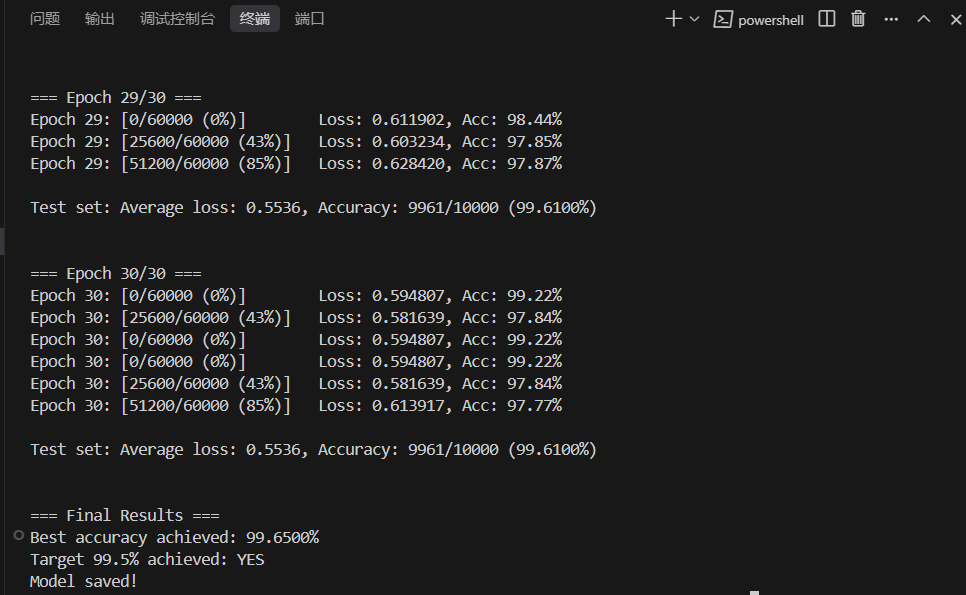
\includegraphics[width=0.9\textwidth]{result.png}
    \caption{模型训练过程收敛结果}
    \label{fig:result}
\end{figure}

根据训练日志,关键节点的数据如下:

\begin{itemize}
    \item \textbf{初步收敛 (Epoch 6)}: 准确率达到 \textbf{99.28\%},已超越传统方法。
    \item \textbf{达成目标 (Epoch 12)}: 准确率首次达到 \textbf{99.50\%},完成了项目的基本目标。
    \item \textbf{性能顶峰 (Epoch 21)}: 准确率达到本次实验的最高值——\textbf{99.65\%}。
    \item \textbf{后期稳定性}: 在训练的最后阶段(22-30 Epochs),准确率始终稳定在 99.6\% 以上的高水平,未见明显下降,表明模型具有良好的泛化能力,并未出现严重过拟合。
\end{itemize}

\textbf{最终最佳准确率:99.65\%},这一结果有力地证明了本研究所采用的综合优化策略的有效性。

\section{结论 (Conclusion)}

本研究成功设计并实现了一个高性能的深度卷积神经网络,在标准的 MNIST 手写数字识别任务上取得了 99.65\% 的测试准确率。这一成果的取得,归功于对一系列现代深度学习技术的系统性集成与应用,包括但不限于深度网络设计、复合数据增强、标签平滑正则化、分层学习率以及高效的训练策略。实验过程不仅验证了这些单项技术的有效性,更展示了将它们有机结合后所产生的强大合力。本项目完整地复现了从设定目标、设计方案、编码实现到迭代优化的标准机器学习工程流程,为解决更复杂的计算机视觉问题积累了宝贵的实践经验。

\begin{thebibliography}{9}
    \bibitem{lecun1998} LeCun, Y., Bottou, L., Bengio, Y., \& Haffner, P. (1998). Gradient-based learning applied to document recognition. \textit{Proceedings of the IEEE, 86(11)}, 2278-2324.
    \bibitem{szegedy2016} Szegedy, C., Vanhoucke, V., Ioffe, S., Shlens, J., \& Wojna, Z. (2016). Rethinking the Inception Architecture for Computer Vision. \textit{Proceedings of the IEEE conference on computer vision and pattern recognition}, 2818-2826.
    \bibitem{loshchilov2017} Loshchilov, I., \& Hutter, F. (2017). Decoupled Weight Decay Regularization. \textit{arXiv preprint arXiv:1711.05101}.
    \bibitem{smith2018} Smith, L. N. (2018). A disciplined approach to neural network hyper-parameters: Part 1 -- learning rate, batch size, momentum, and weight decay. \textit{arXiv preprint arXiv:1803.09820}.
\end{thebibliography}

\end{document} 